%%%%%%%%%%%%%%%%%%%%%%%%%%%%%%%%%%%%%%%%%%%%%%%%%%%%%%%%%%%%%%%%%%%%%%%%%%%%%%%%
%%%%%%%%%%%%%%%%%%   Vorlage für eine Abschlussarbeit   %%%%%%%%%%%%%%%%%%%%%%%%
%%%%%%%%%%%%%%%%%%%%%%%%%%%%%%%%%%%%%%%%%%%%%%%%%%%%%%%%%%%%%%%%%%%%%%%%%%%%%%%%

% Erstellt von Maximilian Nöthe, <maximilian.noethe@tu-dortmund.de>
% ausgelegt für lualatex und Biblatex mit biber

% Kompilieren mit
% latexmk --lualatex --output-directory=build thesis.tex
% oder einfach mit:
% make

\documentclass[
  tucolor,       % remove for less green,
  BCOR=12mm,     % 12mm binding corrections, adjust to fit your binding
  parskip=half,  % new paragraphs start with half line vertical space
  open=any,      % chapters start on both odd and even pages
  cleardoublepage=plain,  % no header/footer on blank pages
]{tudothesis}


% Warning, if another latex run is needed
\usepackage[aux]{rerunfilecheck}

% just list chapters and sections in the toc, not subsections or smaller
\setcounter{tocdepth}{1}

%------------------------------------------------------------------------------
%------------------------------ Fonts, Unicode, Language ----------------------
%------------------------------------------------------------------------------
\usepackage{fontspec}
\defaultfontfeatures{Ligatures=TeX}  % -- becomes en-dash etc.

% load english (for abstract) and ngerman language
% the main language has to come last
\usepackage[american, ngerman]{babel}

% intelligent quotation marks, language and nesting sensitive
\usepackage[autostyle]{csquotes}

% microtypographical features, makes the text look nicer on the small scale
\usepackage{microtype}

%------------------------------------------------------------------------------
%------------------------ Math Packages and settings --------------------------
%------------------------------------------------------------------------------

\usepackage{amsmath}
\usepackage{amssymb}
\usepackage{mathtools}

% Enable Unicode-Math and follow the ISO-Standards for typesetting math
\usepackage[
  math-style=ISO,
  bold-style=ISO,
  sans-style=italic,
  nabla=upright,
  partial=upright,
  warnings-off={mathtools-colon,mathtools-overbracket}, % suppress some unnecessary warnings
]{unicode-math}
\setmathfont{Latin Modern Math}

% nice, small fracs for the text with \sfrac{}{}
\usepackage{xfrac}


%------------------------------------------------------------------------------
%---------------------------- Numbers and Units -------------------------------
%------------------------------------------------------------------------------

\usepackage[
  locale=DE,
  separate-uncertainty=true,
  per-mode=symbol-or-fraction,
]{siunitx}

%------------------------------------------------------------------------------
%-------------------------------- tables  -------------------------------------
%------------------------------------------------------------------------------

\usepackage{booktabs}       % \toprule, \midrule, \bottomrule, etc

%------------------------------------------------------------------------------
%-------------------------------- graphics -------------------------------------
%------------------------------------------------------------------------------

\usepackage{graphicx}
% currently broken
% \usepackage{grffile}

% allow figures to be placed in the running text by default:
\usepackage{scrhack}
\usepackage{float}
\floatplacement{figure}{htbp}
\floatplacement{table}{htbp}

% keep figures and tables in the section
\usepackage[section, below]{placeins}

% allows to include PDFs as full pages
\usepackage{pdfpages}

% Set the PDF Version of this document to 1.7 (1.4 is the current default)
% This is needed so that PDFs with Version >1.5 can be included
\pdfvariable minorversion=7

%------------------------------------------------------------------------------
%---------------------- customize list environments ---------------------------
%------------------------------------------------------------------------------

\usepackage{enumitem}

%------------------------------------------------------------------------------
%------------------------------ Bibliographie ---------------------------------
%------------------------------------------------------------------------------

\usepackage[
  backend=biber,   % use modern biber backend
  autolang=hyphen, % load hyphenation rules for if language of bibentry is not
                   % german, has to be loaded with \setotherlanguages
                   % in the references.bib use langid={en} for english sources
]{biblatex}
\addbibresource{references.bib}  % the bib file to use
\DefineBibliographyStrings{german}{andothers = {{et\,al\adddot}}}  % replace u.a. with et al.


% Last packages, do not change order or insert new packages after these ones
\usepackage[pdfusetitle, unicode, linkbordercolor=tugreen, citebordercolor=tugreen]{hyperref}
\usepackage{bookmark}
\usepackage[shortcuts]{extdash}

%------------------------------------------------------------------------------
%-------------------------    Angaben zur Arbeit   ----------------------------
%------------------------------------------------------------------------------

\author{Joel Koch}
\title{Detecting Brain Tumours using a Convolutional Neural Network}
\subtitle{Seminar: Machine Learning for Physicists}
\date{31.07.2024}
% \birthplace{Castrop-Rauxel}
\chair{Experimental Physics IV}
\division{Faculty Physics}

% tu logo on top of the titlepage
\titlehead{\includegraphics[height=1.5cm]{../logo_engl.pdf}}

\begin{document}
\frontmatter
\maketitle

% Gutachterseite
% \makecorrectorpage

% hier beginnt der Vorspann, nummeriert in römischen Zahlen
% \thispagestyle{plain}

\section*{Kurzfassung}
Hier steht eine Kurzfassung der Arbeit in deutscher Sprache inklusive der Zusammenfassung der
Ergebnisse.
Zusammen mit der englischen Zusammenfassung muss sie auf diese Seite passen.

\section*{Abstract}
\begin{foreignlanguage}{english}
The abstract is a short summary of the thesis in English, together with the German summary it has to fit on this page.
\end{foreignlanguage}

\tableofcontents

\mainmatter
% Hier beginnt der Inhalt mit Seite 1 in arabischen Ziffern
\chapter{Introduction}
\label{cha:introduction}

To detect brain tumours and classify them into malignant and benign, is a vital challenge in the field of medical diagnostics. 
Accurate and timely diagnosis is essential for effective treatment planning and improving the patient's health.
Traditional methods for diagnosing brain tumours are biopsies or manually evaluating medical images like magnetic resonance imaging (MRI) scans \cite{CancerResearUK}.
These methods are time-consuming, expensive, and can be error-prone. 
With advancements in the field of machine learning, it is possible to automate the process of diagnosing brain tumours using machine learning techniques. %convolutional neural networks (CNNs).
To use machine learning, the brain tumour which is to be classified as malignant or benign, needs to be analysed by a doctor into certain features.
These features can be extracted from MRI scans and used as input for a machine-learning model.
To overcome this analysis step, a neural network can be trained on the MRI scans themselves.
A task such as this is known as image classification.
Convolutional neural networks (CNNs) are a type of artificial neural network that is well-suited for image classification tasks, by applying filters to input images to detect patterns.

A CNN to classify brain tumours in MRI scans as malignant or benign is developed in this work.
This model is compared to binary classification models to evaluate its performance, such as logistic regression, support vector machines, and k-nearest neighbours.
The metric used to evaluate the models is the recall score, as it is important to detect malignant tumours correctly.

The dataset used in this work is the "Brain Tumor" dataset from Kaggle \cite{jakesh_bohaju_2020}.
It contains 3762 images with labels that can be used for the CNN.
It also contains five first-order and eight second-order features that can be used for the binary classification methods and described later.
% The first-order features are mean, variance, skewness, kurtosis, and entropy.
% The second-order features are contrast, energy, angular second moment (ASM), entropy, homogeneity, dissimilarity, correlation, and coarseness.
The dataset runs under the Creative Commons license, which allows for sharing and adapting the dataset for non-commercial purposes \href{https://creativecommons.org/licenses/by-nc-sa/4.0/}{(CC BY-NC-SA 4.0)}. 
% The CNN is trained on the images from the dataset, and the binary classification models are trained on the features extracted from the images.

The CNN is explained in more detail in chapter \ref{cha:CNN}, where the network architecture, the initial model, the hyperparameter optimization, and the final model are discussed.
The binary classification models are explained in chapter \ref{cha:alternative_methods} and a comparison between the CNN and the binary classification models is made in section \ref{sec:comparison}.
% A comparison between the CNN and the binary classification models is made in section \ref{sec:comparison}.
A discussion and an outlook are given in chapter \ref{cha:conclusion}. 
The code can be found in the corresponding GitHub repository \cite{project} or directly via the \href{https://github.com/joeyko2706/MachineLearning24/tree/main}{link}.

% \section{Dataset}
% \label{sec:dataset}



% \cite{tensorflow}
% \begin{figure}[H]
%     \centering
%     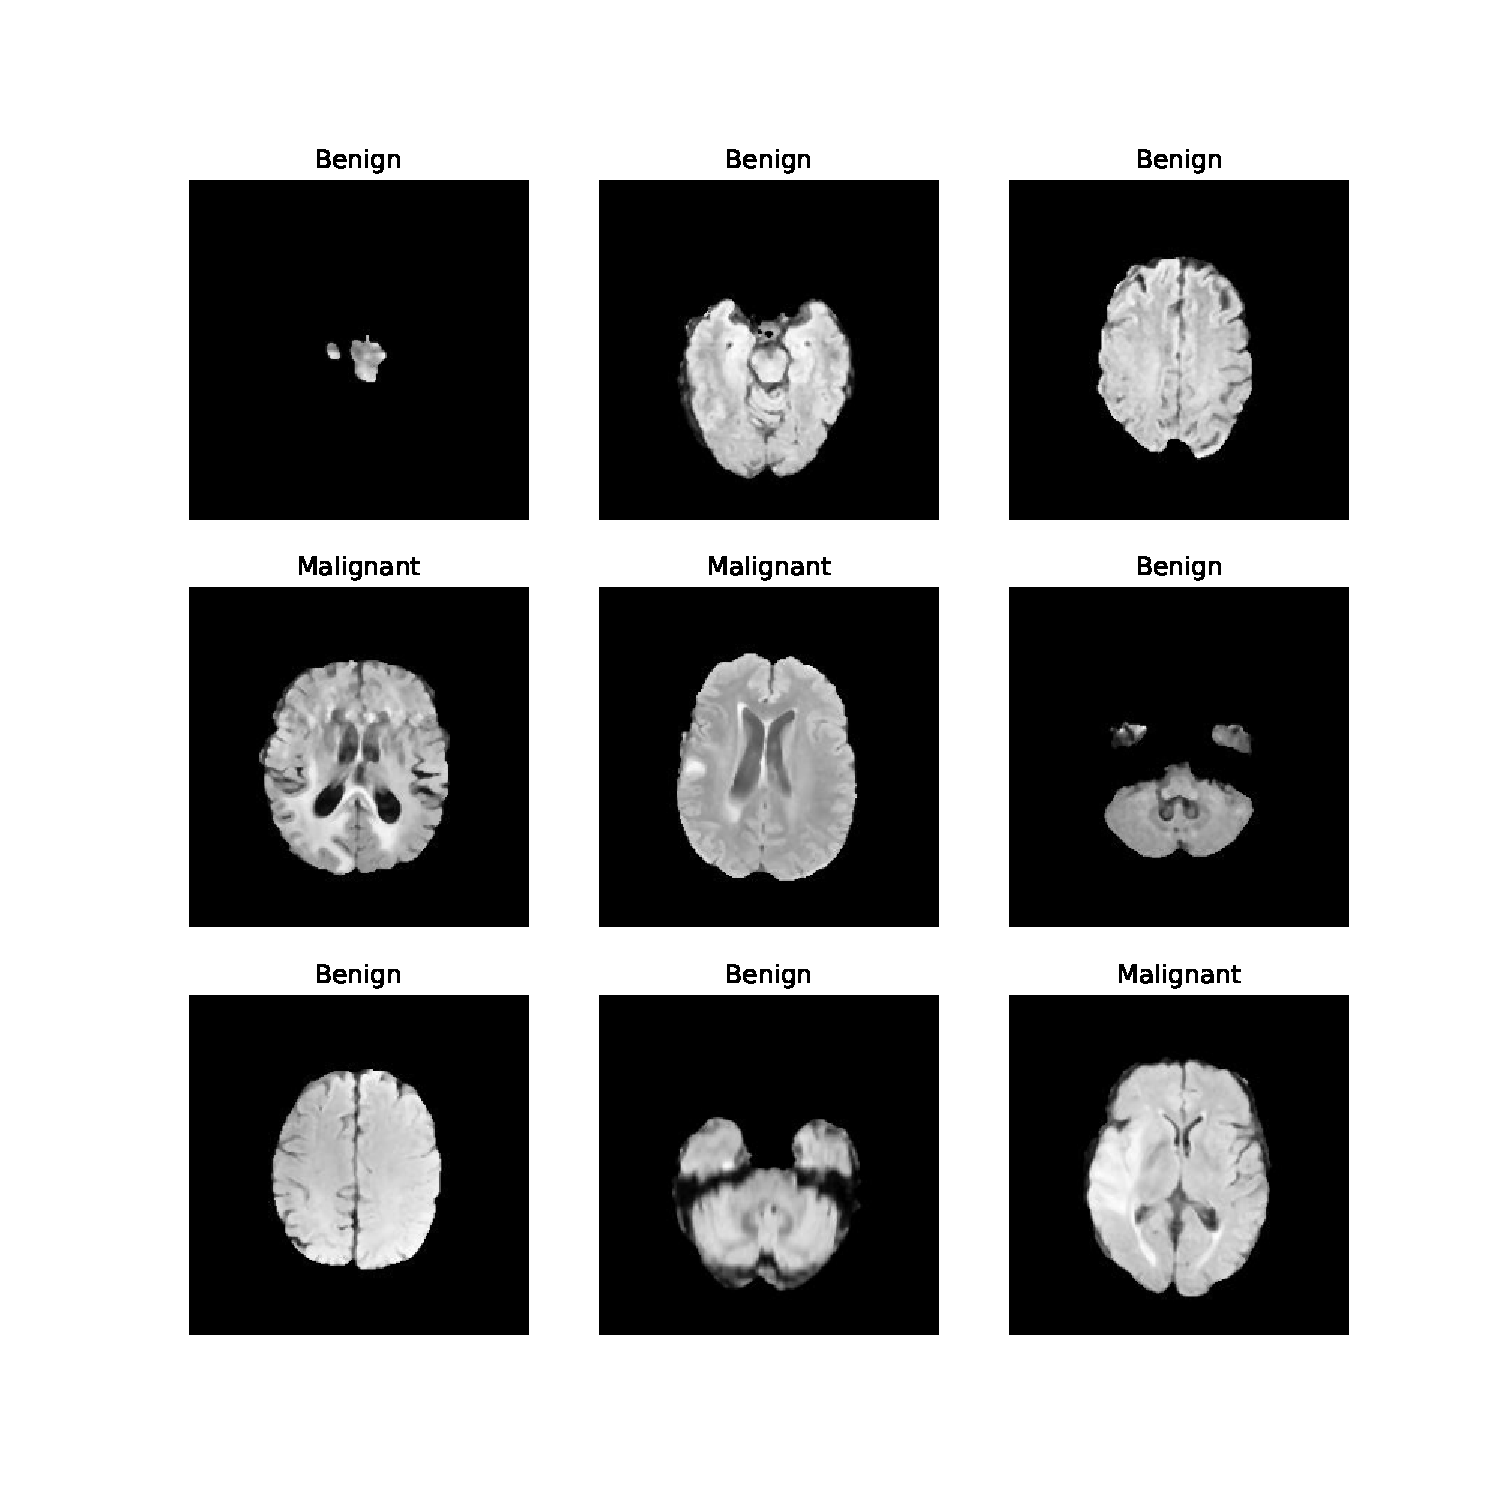
\includegraphics[width=.8\textwidth]{plots/tumor_images.pdf}
%     \caption{Malignant and benign tumour images from the dataset.}
%     \label{fig:tumorImages}
% \end{figure}

\chapter{Network Architecture}
\label{sec:architecture}

\chapter{Results}
\label{sec:results}



\begin{figure}[H]
    \centering
    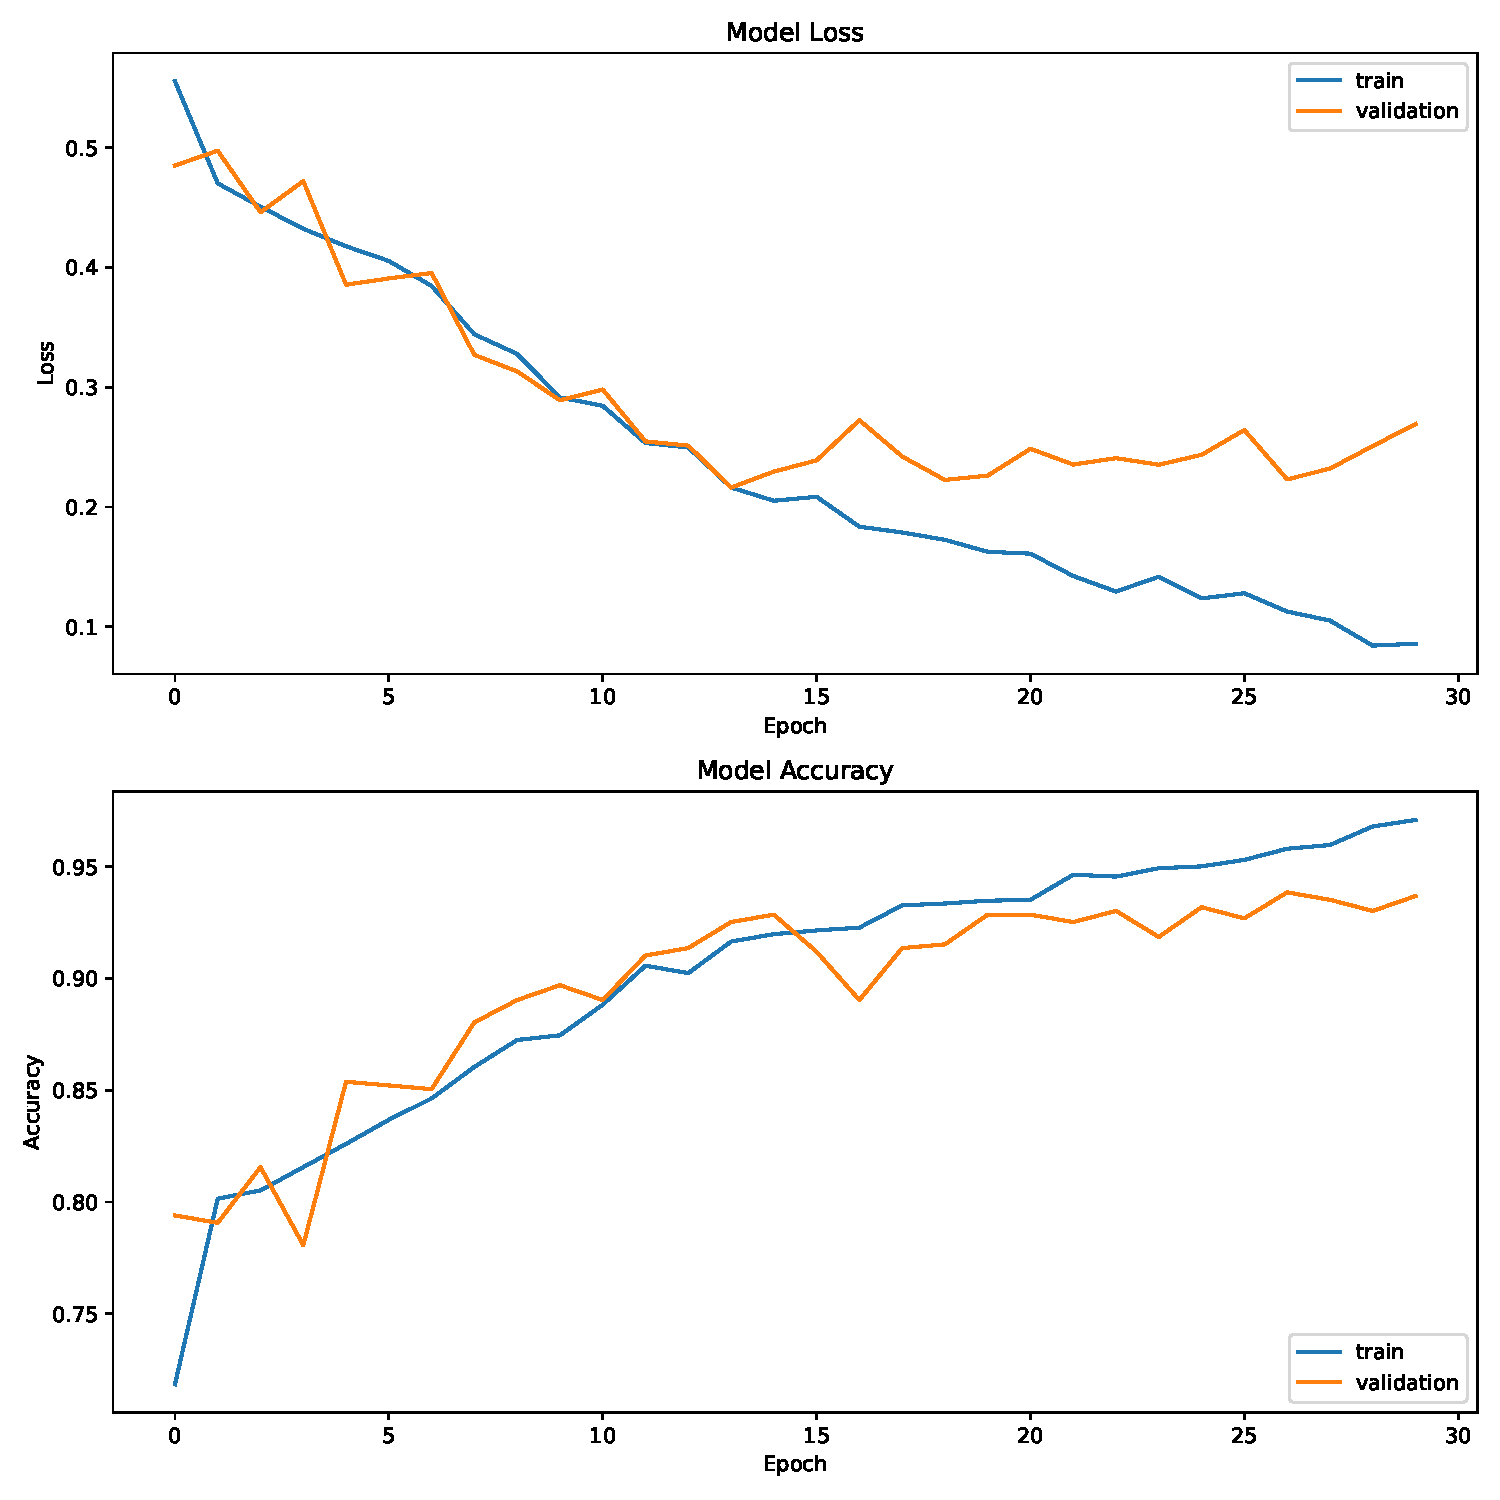
\includegraphics[width=.7\textwidth]{plots/CNN_history.pdf}
    \caption{Accuracy- and loss-curves for the initial CNN.}
    \label{fig:learningCurveInitial}
\end{figure}


\begin{figure}[H]
    \centering
    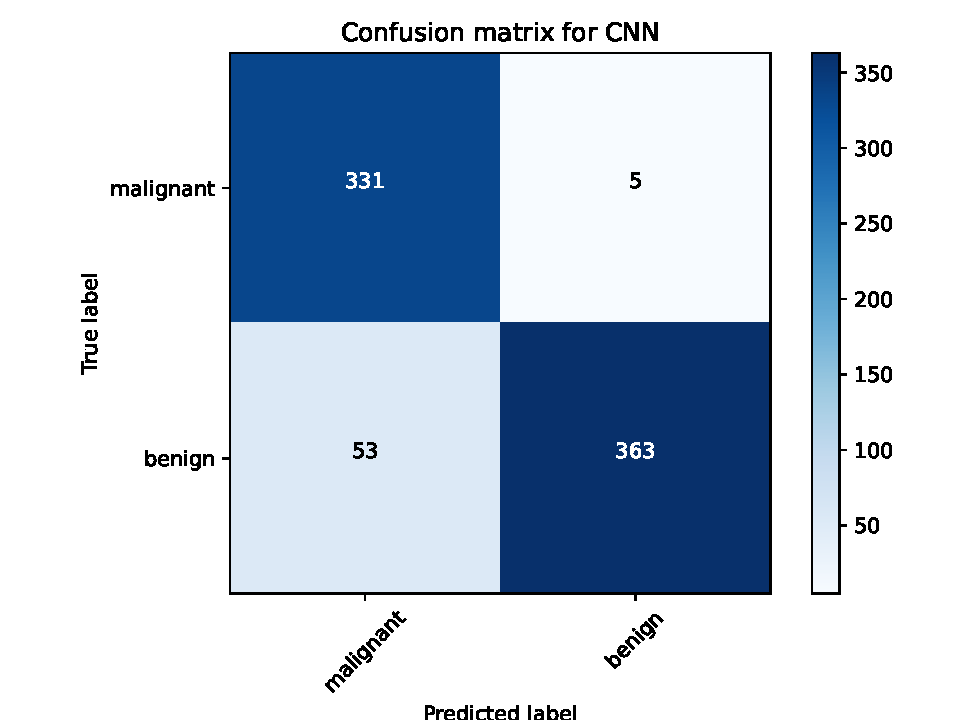
\includegraphics[width=.5\textwidth]{plots/confusion_matrix_CNN.pdf}
    \caption{Confusion matrix for the initial CNN.}
    \label{fig:confusionMatrixInitial}
\end{figure}



\section{Hyperparameter Optimization}
\label{sec:hyperparameter}



\begin{figure}[H]
    \centering
    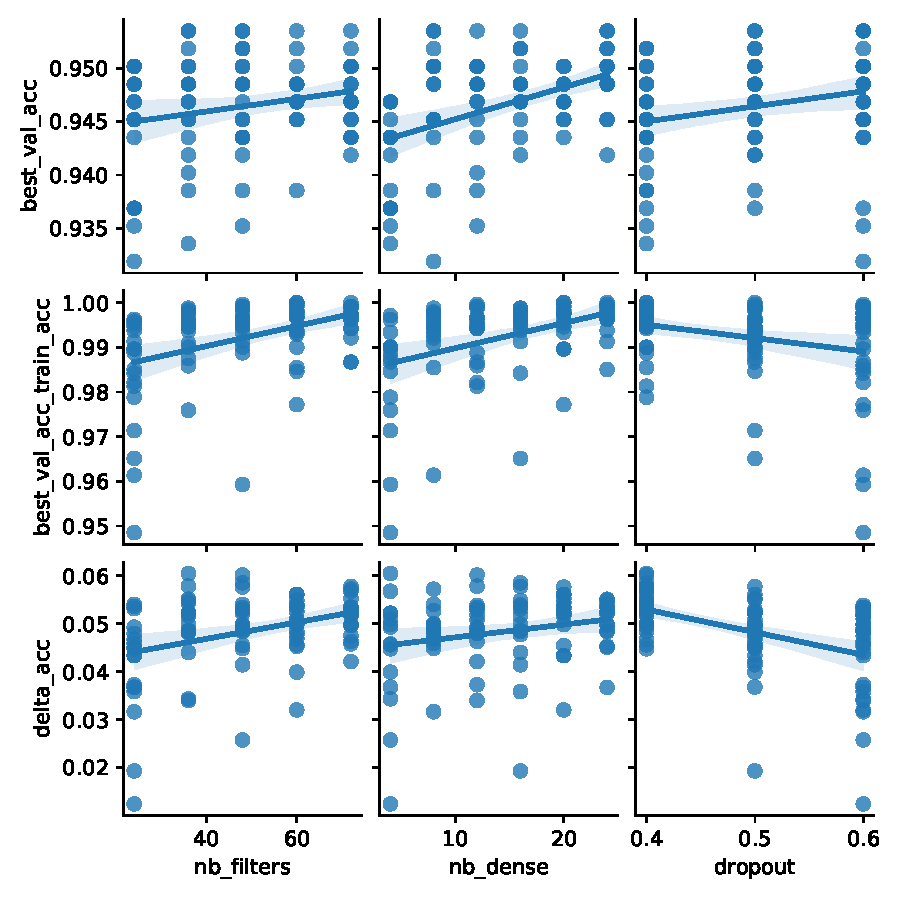
\includegraphics[width=0.7\textwidth]{plots/pairplot.pdf}
    \caption{Hyperparameter testing using gridsearch.}
    \label{fig:gridsearch}
\end{figure}

\begin{figure}[H]
    \centering
    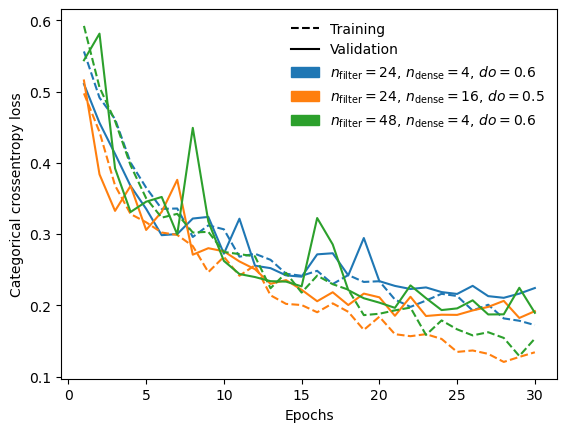
\includegraphics[width=0.7\textwidth]{plots/SmallestDelta_LearningCurves.png}
    \caption{Learning curves of the models from the gridsearch with the least difference between training and validation.}
    \label{fig:SmallestDelta_LearningCurves}
\end{figure}


\begin{figure}[H]
    \centering
    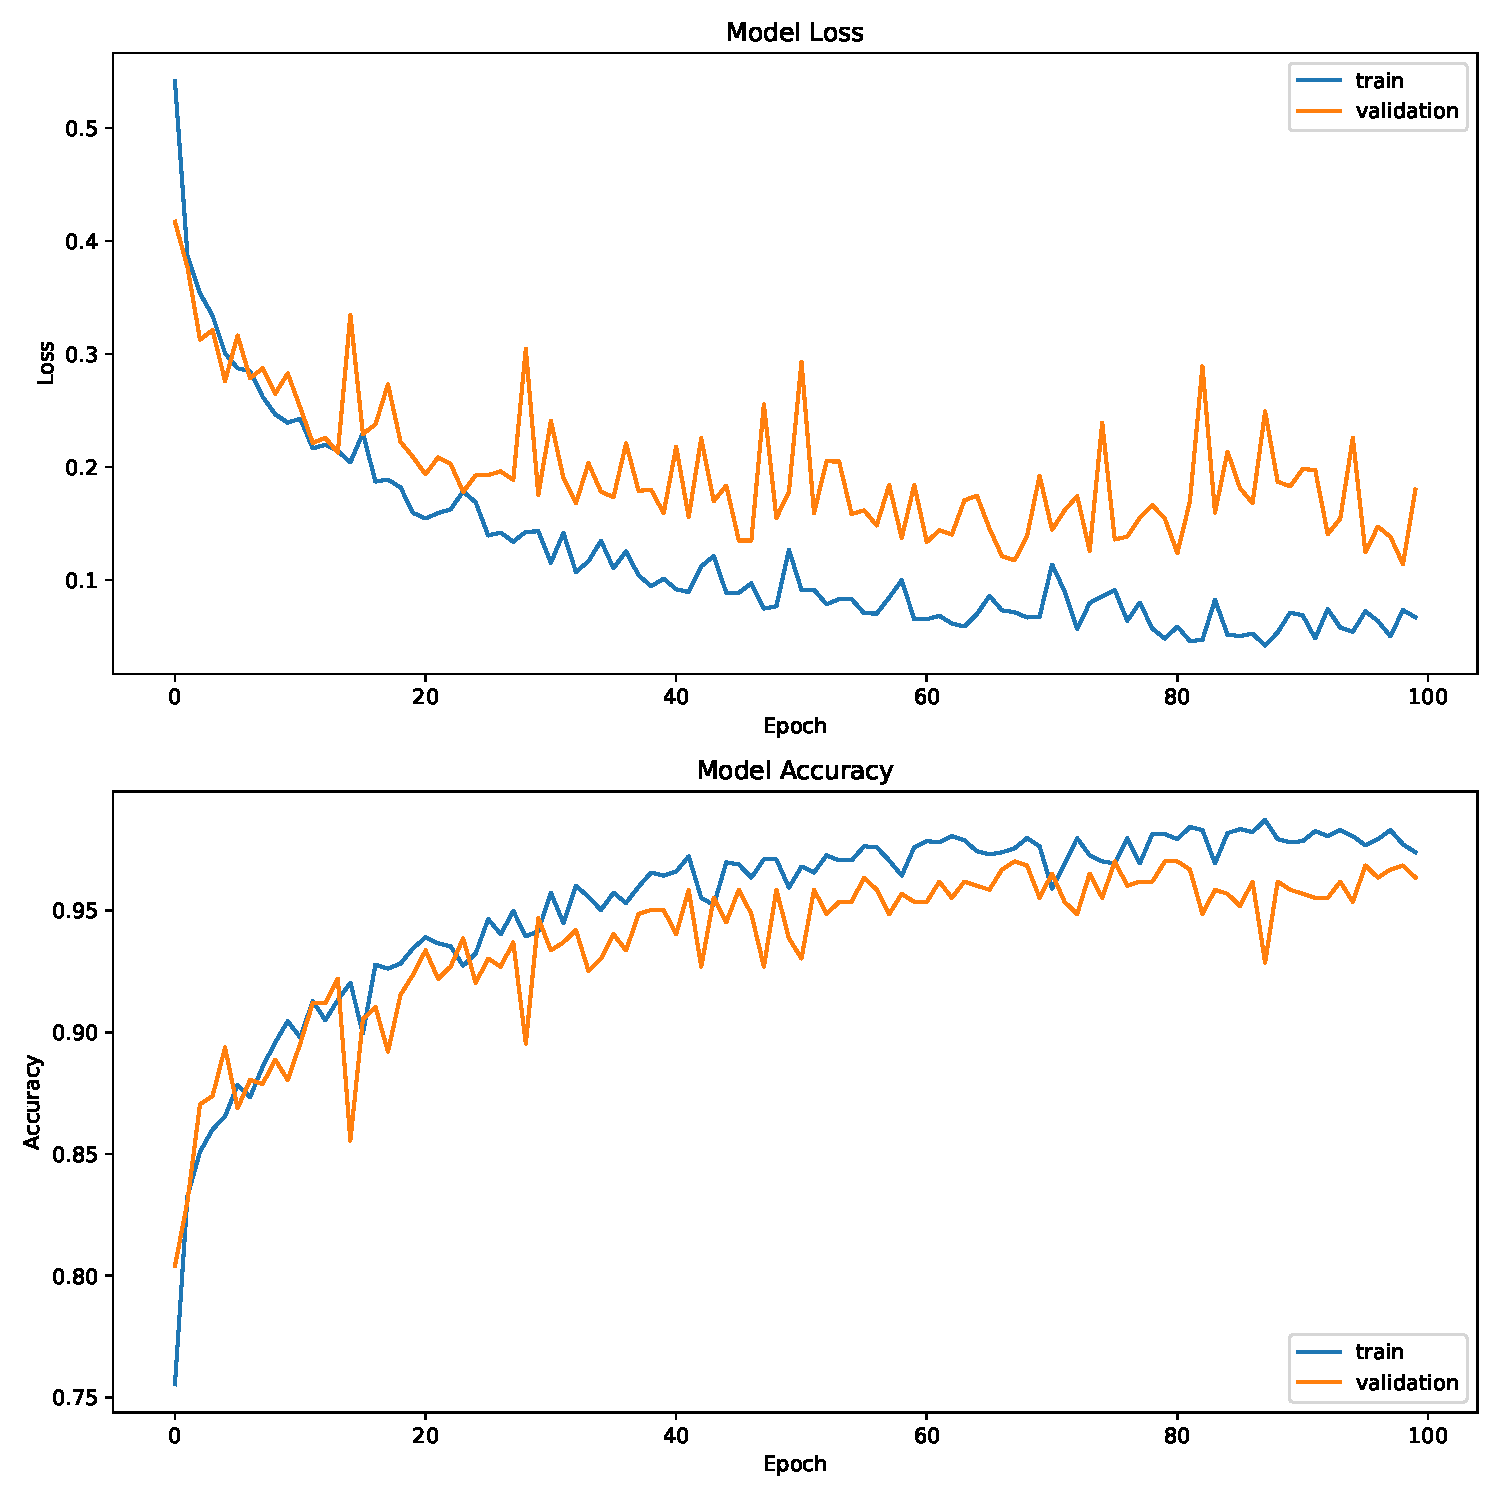
\includegraphics[width=.7\textwidth]{plots/history.pdf}
    \caption{Accuracy- and loss-curves for the initial CNN.}
    \label{fig:learningCurveFinal}
\end{figure}


\begin{figure}[H]
    \centering
    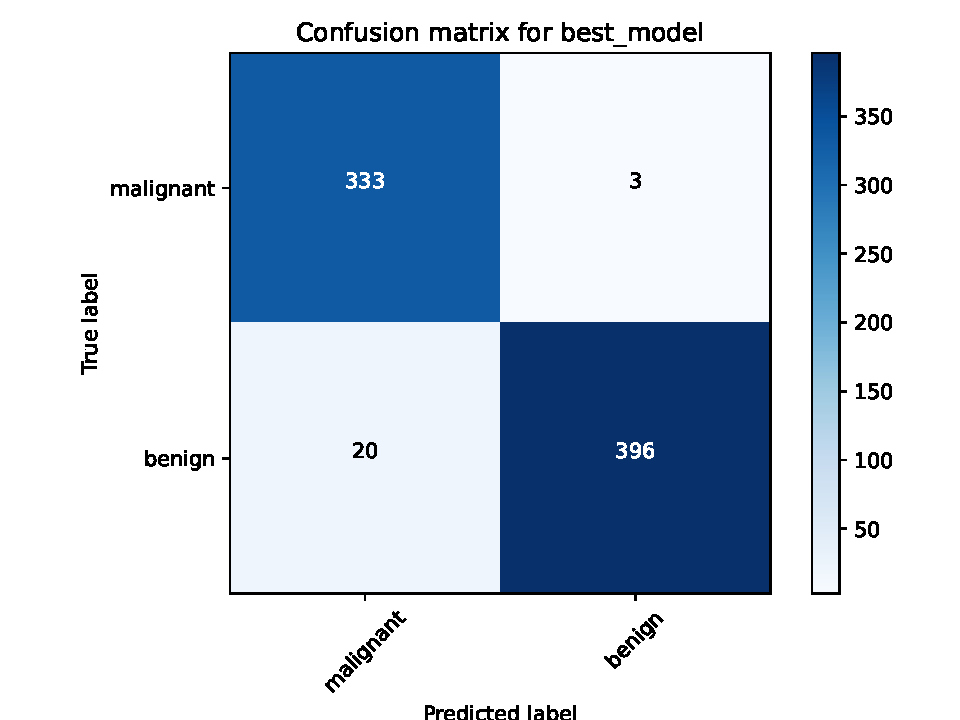
\includegraphics[width=.5\textwidth]{plots/confusion_matrix_best_model.pdf}
    \caption{Confusion matrix for the initial CNN.}
    \label{fig:confusionMatrixFinal}
\end{figure}
\chapter{Alternative Methods}
\label{cha:alternative_methods}



\section{Comparison to the CNN}
\label{sec:comparison}

\begin{table}[H]
    \centering
    \caption{Comparison of the alternative methods to the initial and the final CNN.}
    \label{tab:comparisonTable}
    \begin{tabular}{c | c c c c c c c}
        \toprule
        model & recall & accuracy & precision & f1-score & $R^2$-score & Mean Squared Error \\%& Mean Absolute Error \\
        \midrule
        SVM & 0.9617 & 0.9801 & 0.9939 & 0.9775 & 0.9195 & 0.0199 \\
        LR & 0.9617 & 0.9788 & 0.9909 & 0.9760 & 0.9141 & 0.02124 \\
        kNN & 0.9469 & 0.9761 & 1.0 & 0.97273 & 0.9034 & 0.0239 \\
        CNN & 0.8726 & 0.9229 & 0.9864 & 0.926 & 0.688 & 0.0771 \\
        best model & 0.9519 & 0.9694 & 0.9925 & 0.9718 & 0.8763 \\ 
        \bottomrule
    \end{tabular}
\end{table}


% \appendix
% % Hier beginnt der Anhang, nummeriert in lateinischen Buchstaben
% \chapter{Appendix}
\label{cha:appendix}

\section{Data Exploration}
\label{sec:DataExploration}

% \begin{figure}[H]
%     \centering
%     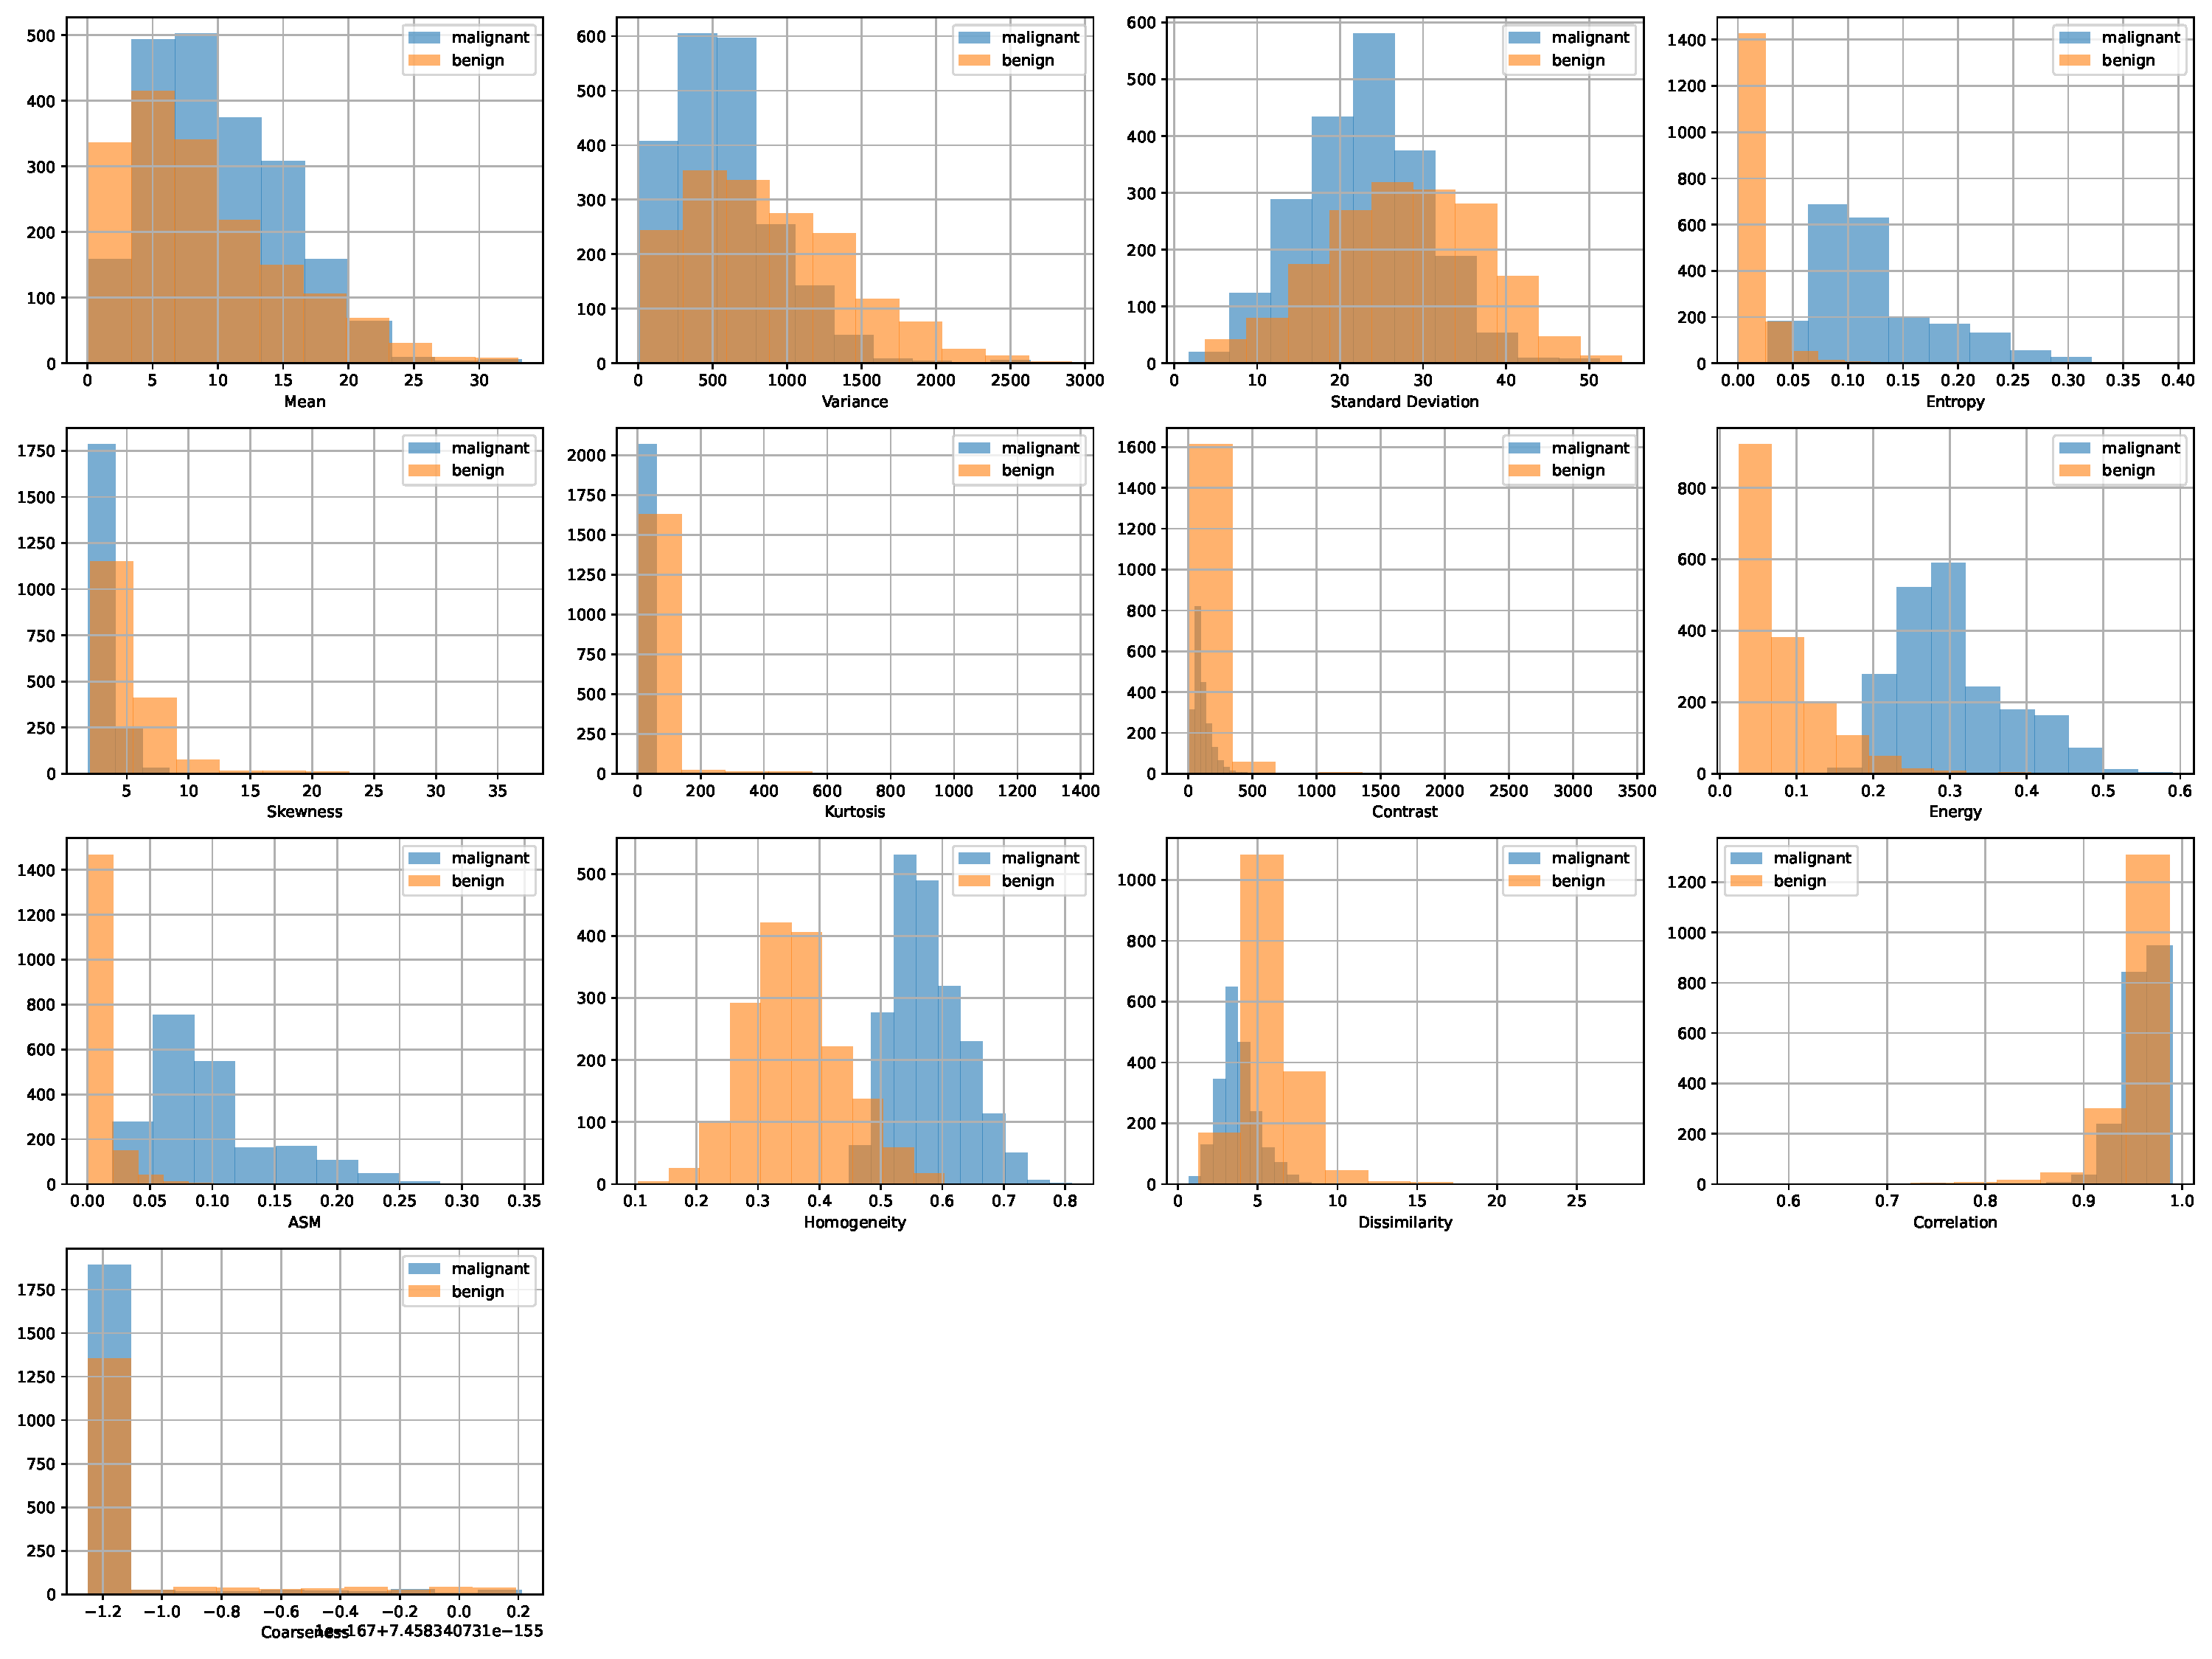
\includegraphics[width=.8\textwidth]{plots/benign_malignant_comparison.pdf}
%     \caption{Comparison between benign and malignant brain tumours for the first- and second-order features.}
%     \label{fig:benign_malignant_comparison}
% \end{figure}

The correlation and scatter matrix of the first- and second-order features are shown in figures \ref{fig:correlation} and \ref{fig:scatter_matrix} respectively.

\begin{figure}[H]
    \centering
    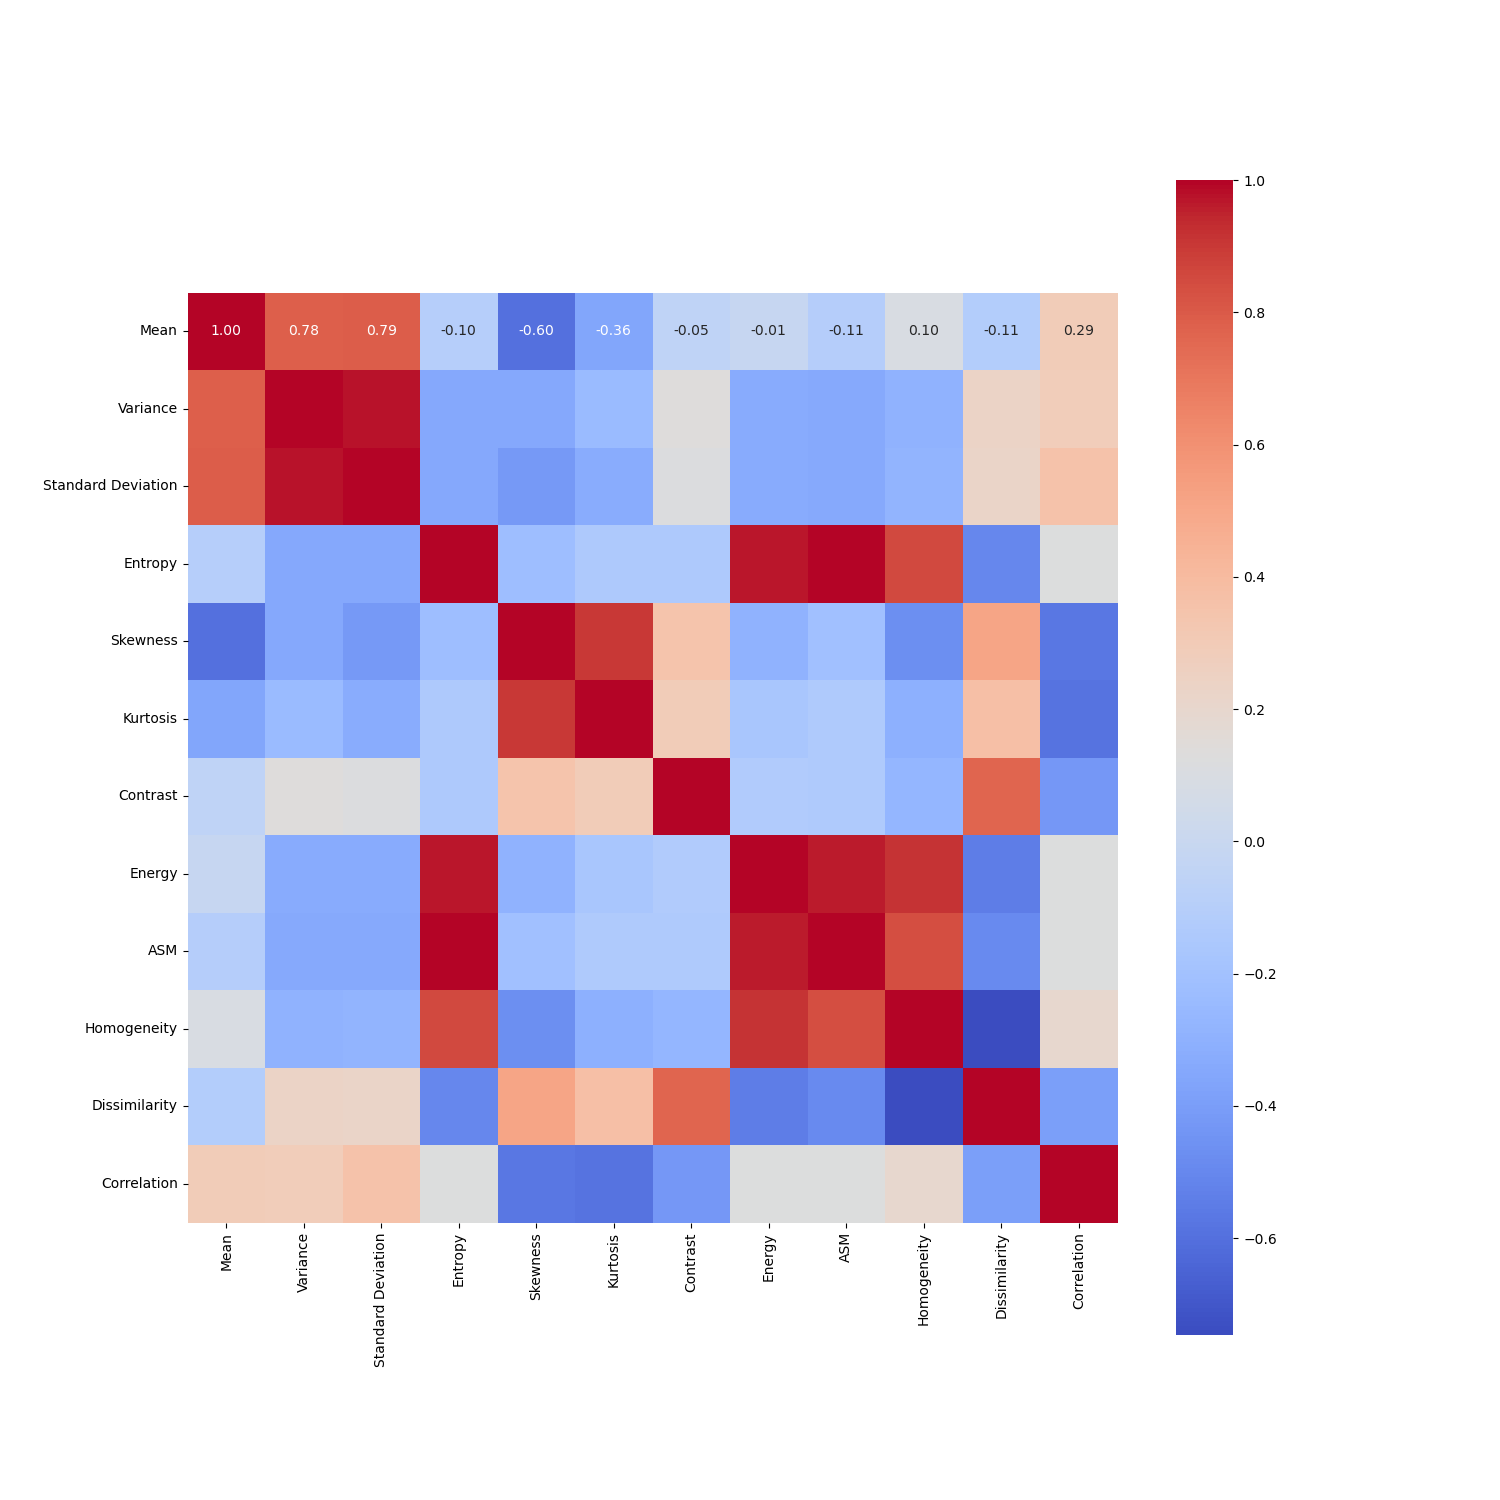
\includegraphics[width=.8\textwidth]{plots/correlation.png}
    \caption{Correlation of the first- and second-order features.}
    \label{fig:correlation}
\end{figure}

\begin{figure}[H]
    \centering
    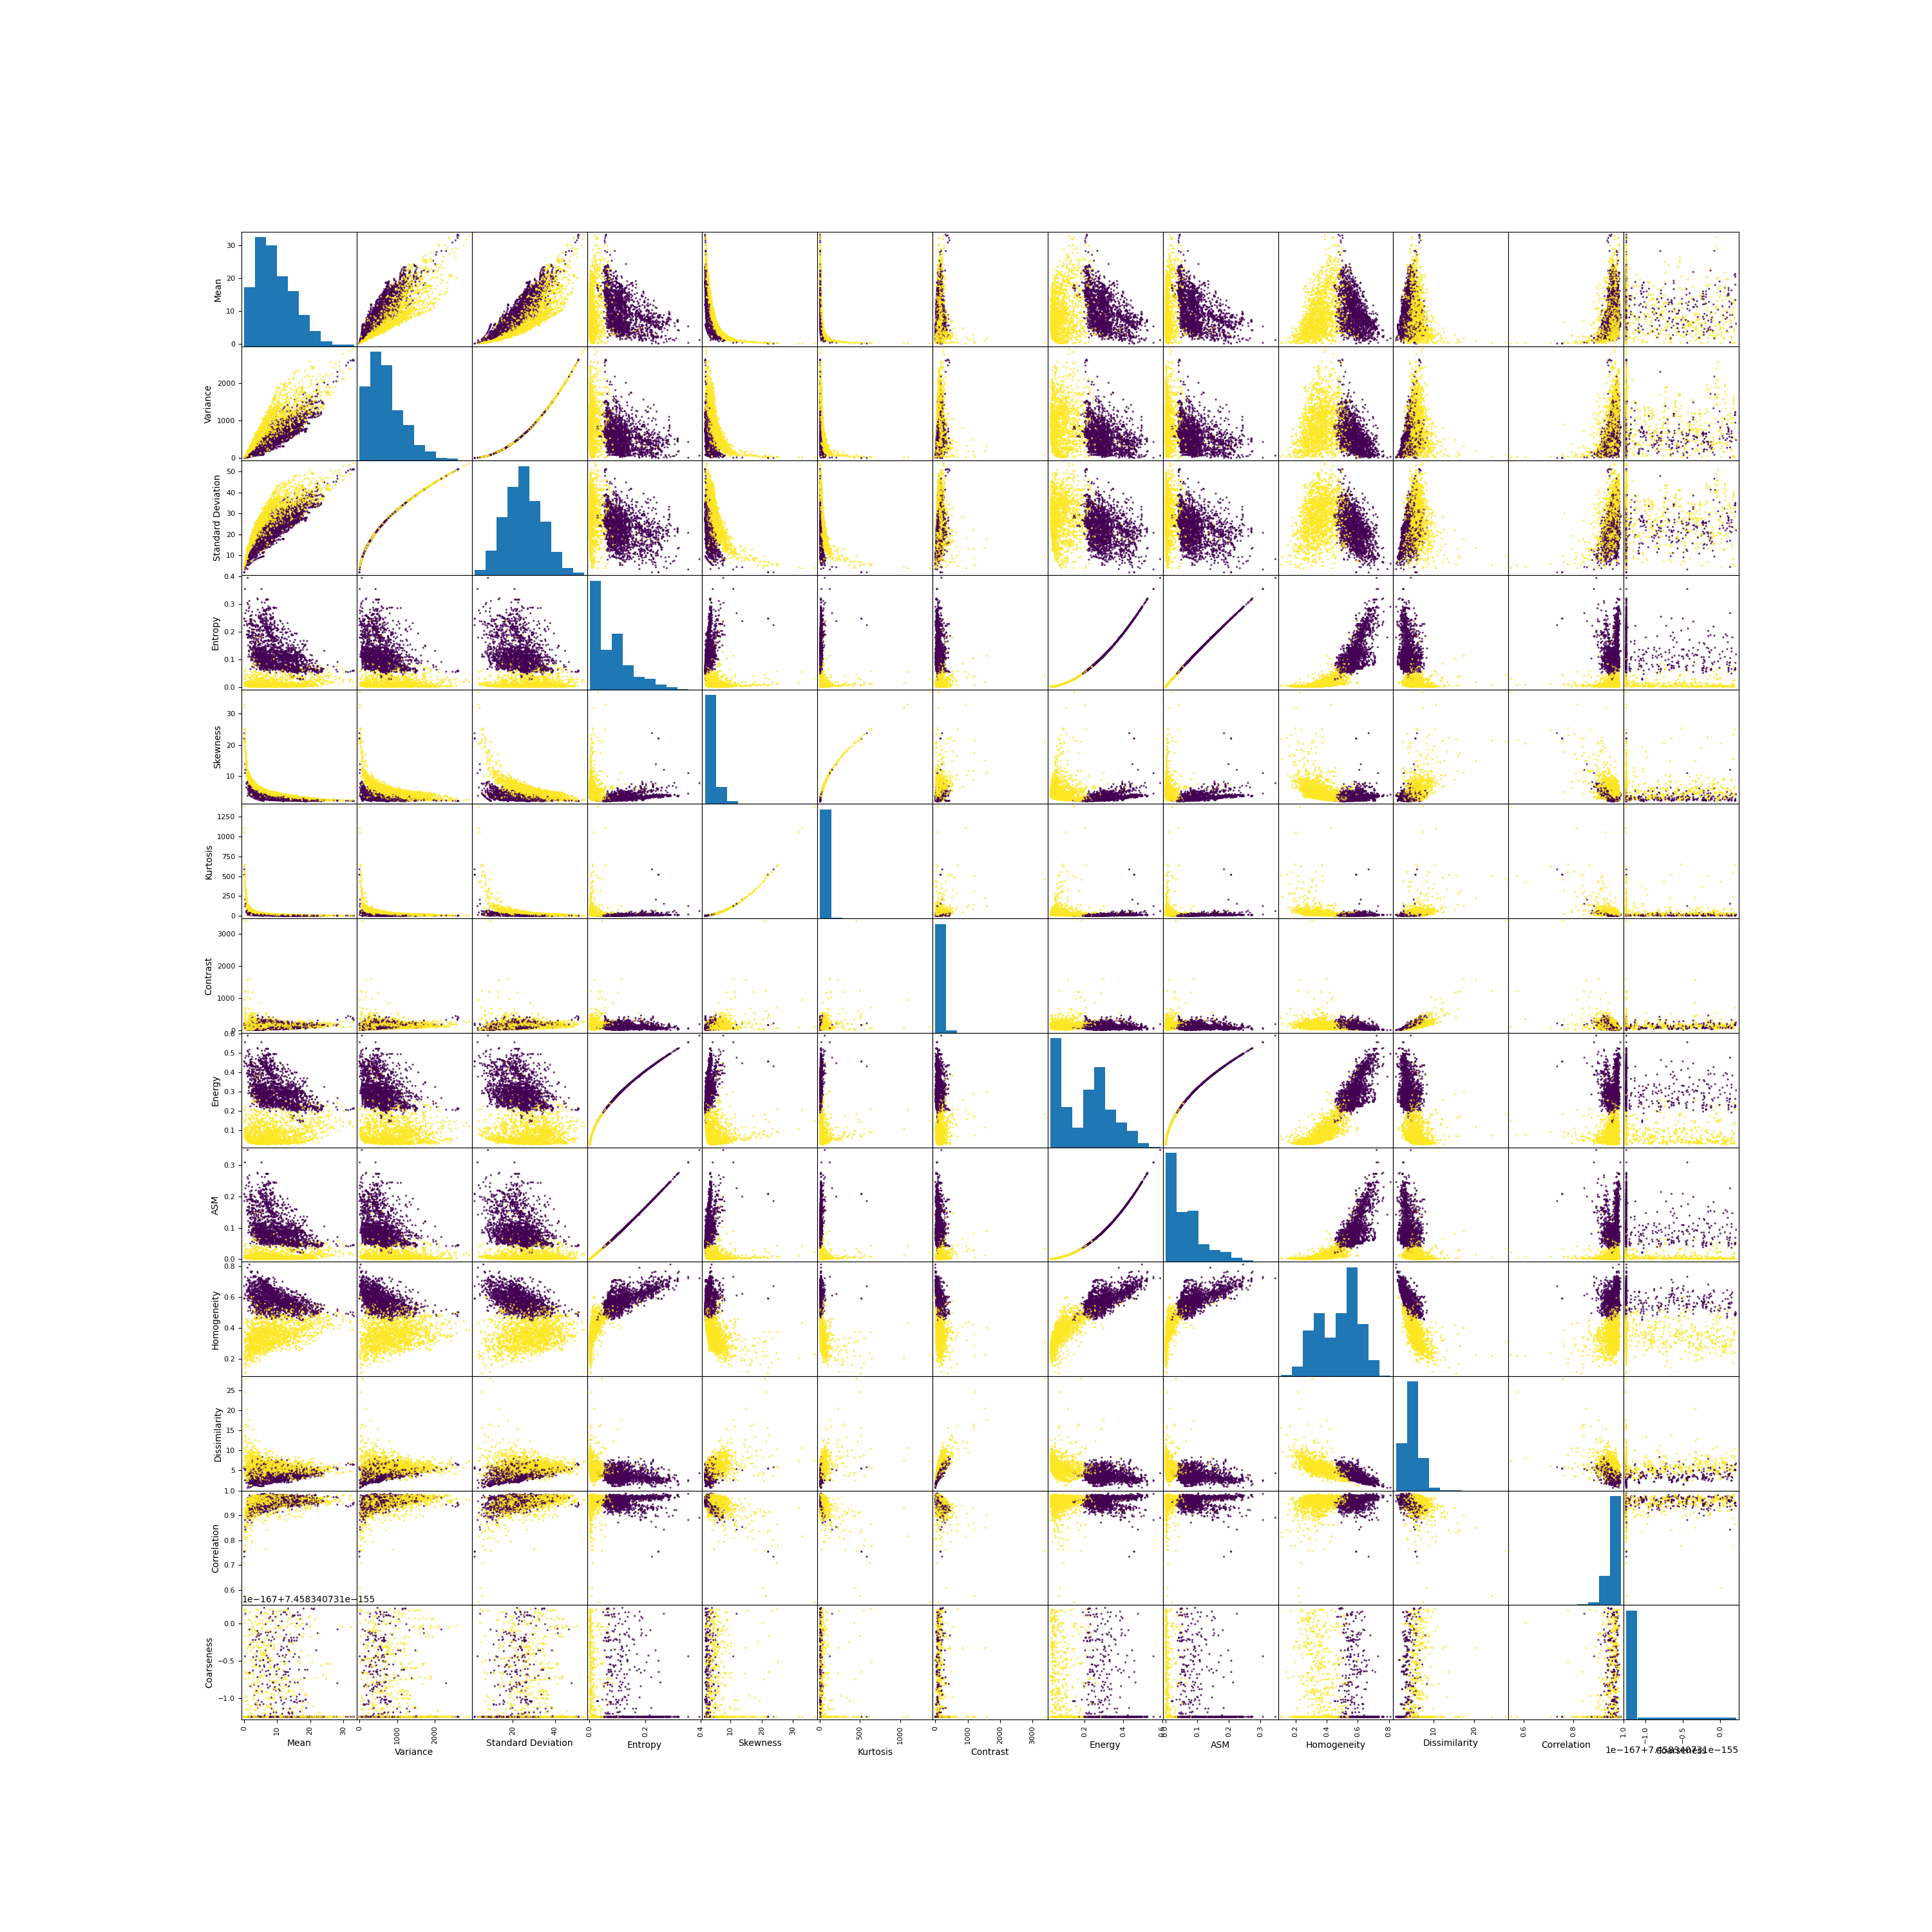
\includegraphics[width=.8\textwidth]{plots/scatter_matrix.png}
    \caption{Scatter matrix of the first- and second-order features.}
    \label{fig:scatter_matrix}
\end{figure}


\section{First Gridsearch Hyperparameter Tests}
\label{sec:FirstGridsearchHyperparameterTests}

Figure \ref{fig:FirstHyperparameterTests} shows the first hyperparameter tests using gridsearch.
This hyperparameter test led to the test, which is described in section \ref{sec:hyperparameter}.
The main goal was to reduce the overfitting, which is why the delta between the training and validation loss was used as the main metric. 
Because the dropout rate decreased the delta between the training and validation loss so much, it was decided to increase the dropout range to 0.6 in the next test.
Because the number of dense units did not have an impact on the delta, a higher range was chosen for the next test.
The range of the number of filters in the convolutional layers was not increased as the delta increased with the number of filters.
There was only taken more data for the next test by using more filters in the same range.

\begin{figure}[H]
    \centering
    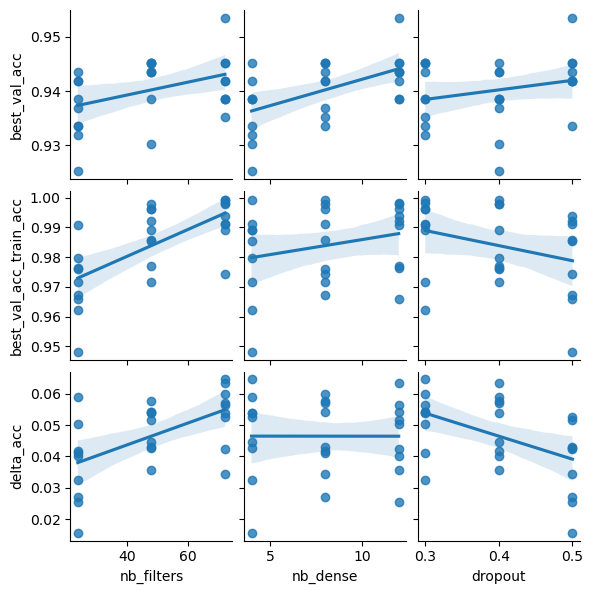
\includegraphics[width=.8\textwidth]{plots/FirstHyperparameterTests.png}
    \caption{First hyperparameter tests using gridsearch.}
    \label{fig:FirstHyperparameterTests}
\end{figure}



\backmatter
\printbibliography

\cleardoublepage
% From https://www.tu-dortmund.de/studierende/im-studium/pruefungsangelegenheiten/allgemeine-vordrucke/
% 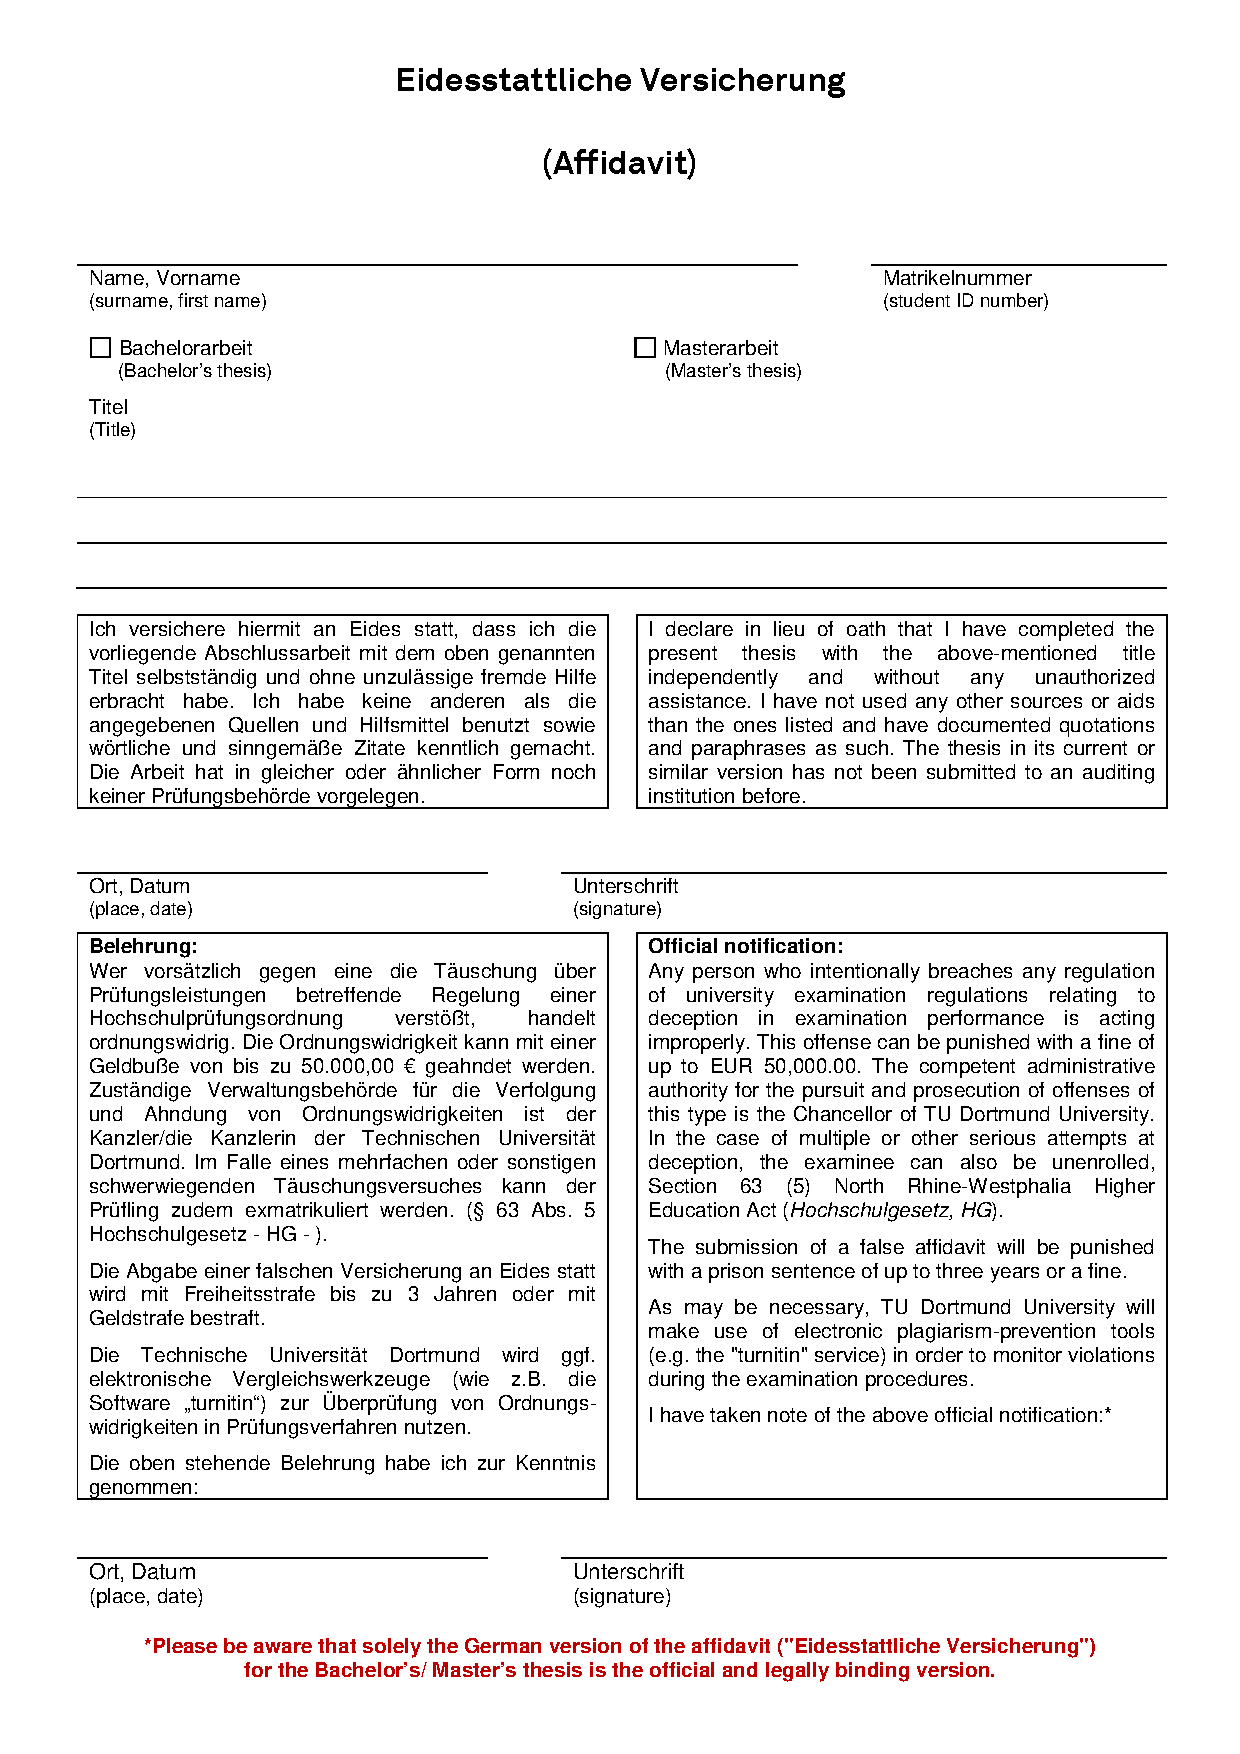
\includepdf{content/Eidesstattliche_Versicherung.pdf}

\end{document}
